\subsection{Herramientas de seguridad adicionales}\label{sec:herramientas-adicionales}

WireGuard es un túnel VPN moderno orientado al rendimiento y la simplicidad operativa. Utiliza criptografía actual, opera sobre UDP, y se integra con facilidad en entornos de campus y acceso remoto. Para su implementación se recomienda: generar pares de claves por dispositivo, definir pares (\textit{peers}) con \texttt{AllowedIPs} específicos, publicar el servicio en el puerto UDP 51820, aplicar reglas de cortafuegos que restrinjan el alcance de las subredes expuestas y habilitar registro de eventos para auditoría.

\begin{figure}[H]
	\centering
	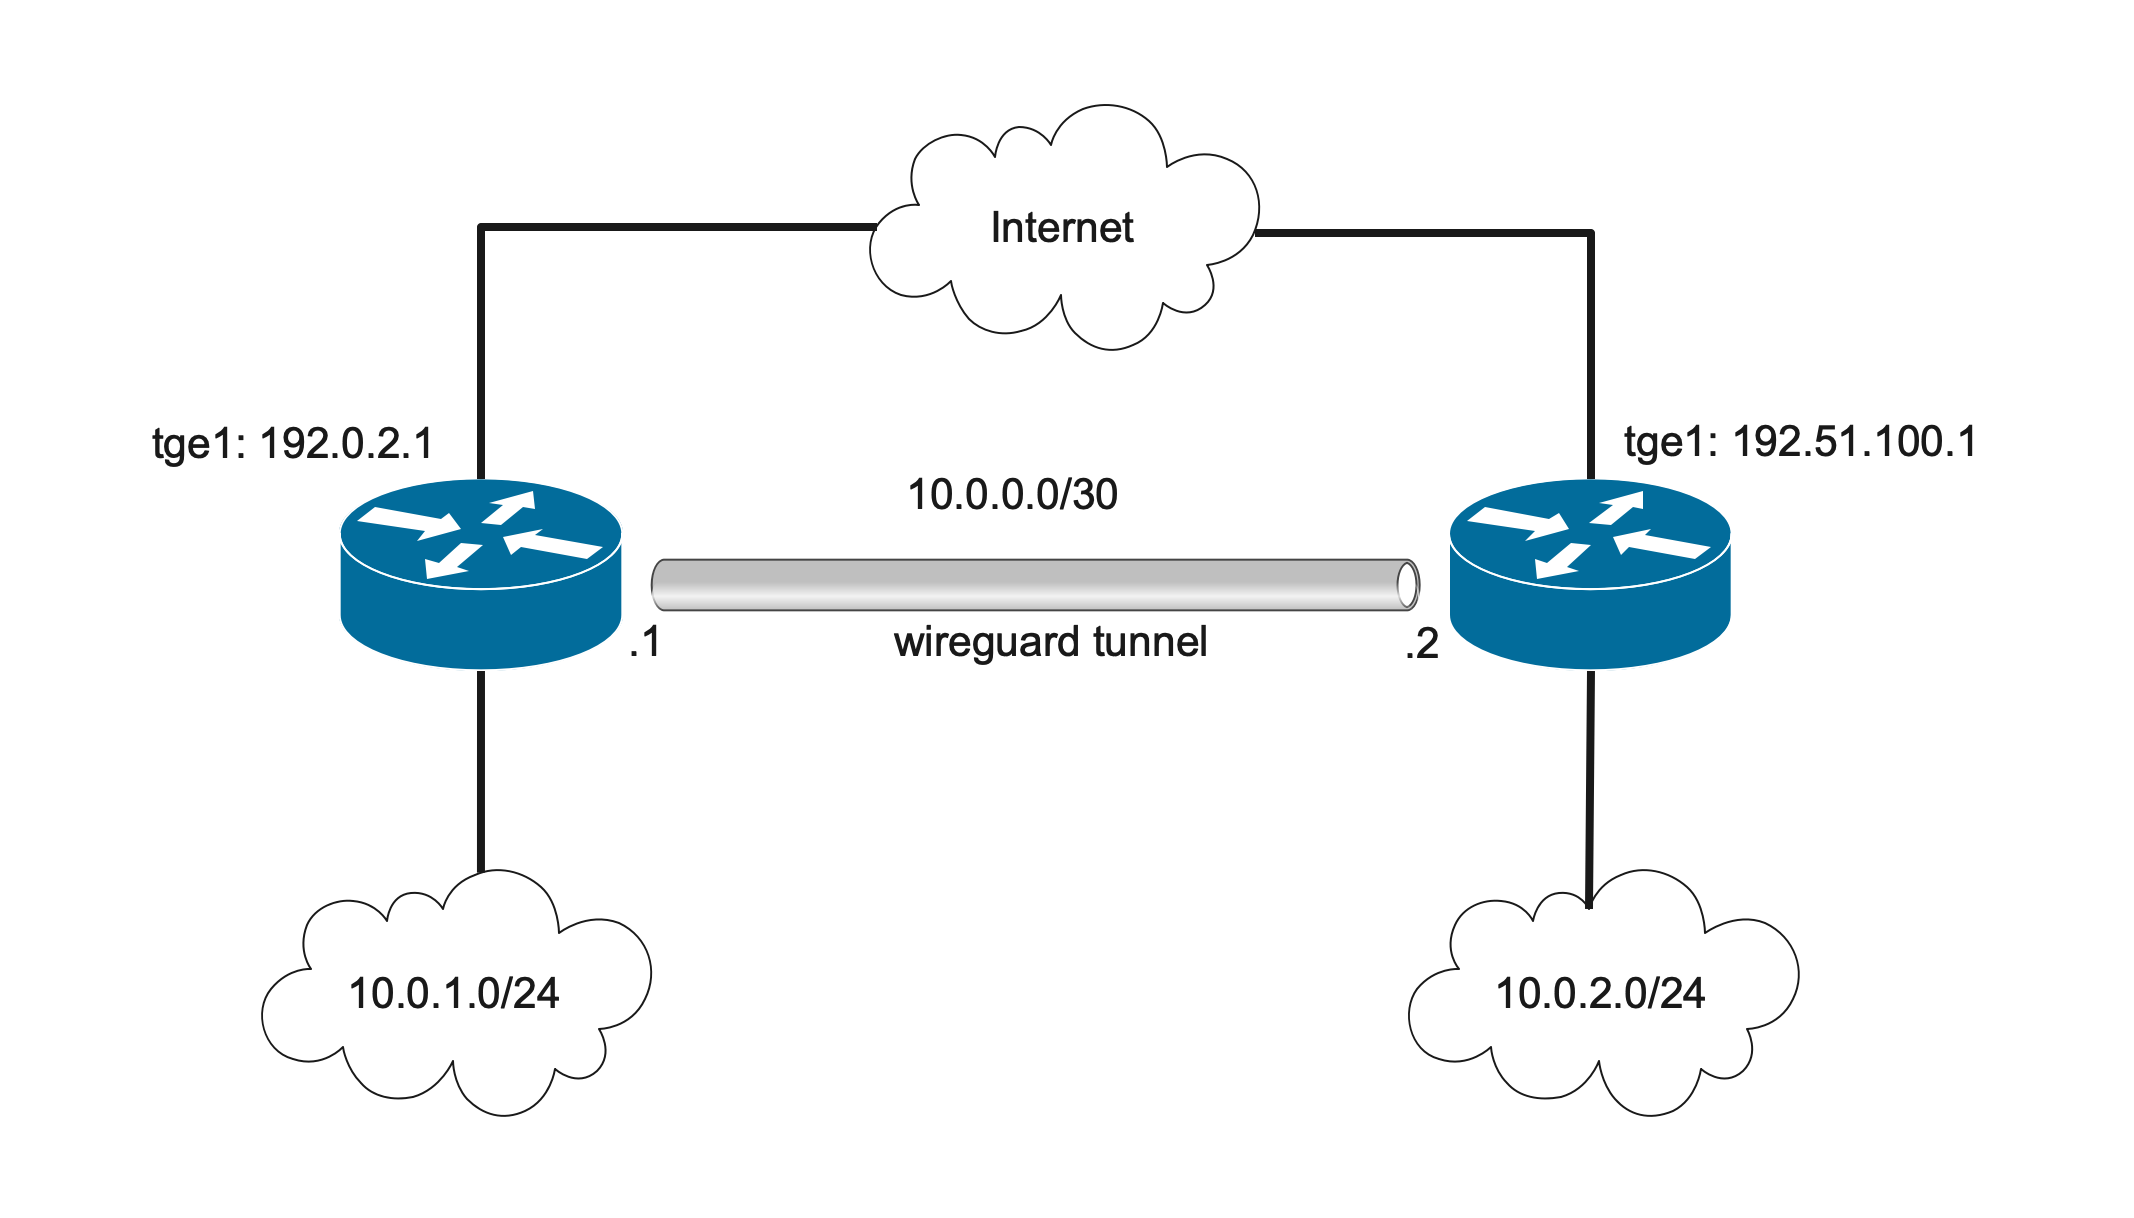
\includegraphics[width=0.9\linewidth]{images/wireguard-example}
	\caption{Ejemplo de topología con WireGuard}\label{fig:wireguard-example}
\end{figure}



Como complemento a la VPN, se sugieren herramientas puntuales para refuerzo defensivo:

- \textit{Suricata} (IDS/IPS): motor de inspección profunda de paquetes que permite detección y prevención de intrusiones, útil en modo espejo (IDS) o en línea (IPS) con reglas actualizadas. Facilita visibilidad sobre patrones anómalos y ataques comunes. 

- \textit{Wazuh} (Antimalware): plataforma de seguridad y monitoreo que integra capacidades de detección de malware, análisis de integridad y gestión de vulnerabilidades. Permite la supervisión continua de endpoints y servidores, generando alertas ante actividades sospechosas. Su arquitectura distribuida facilita la escalabilidad en entornos de red complejos.

\begin{figure}[H]
	\centering
	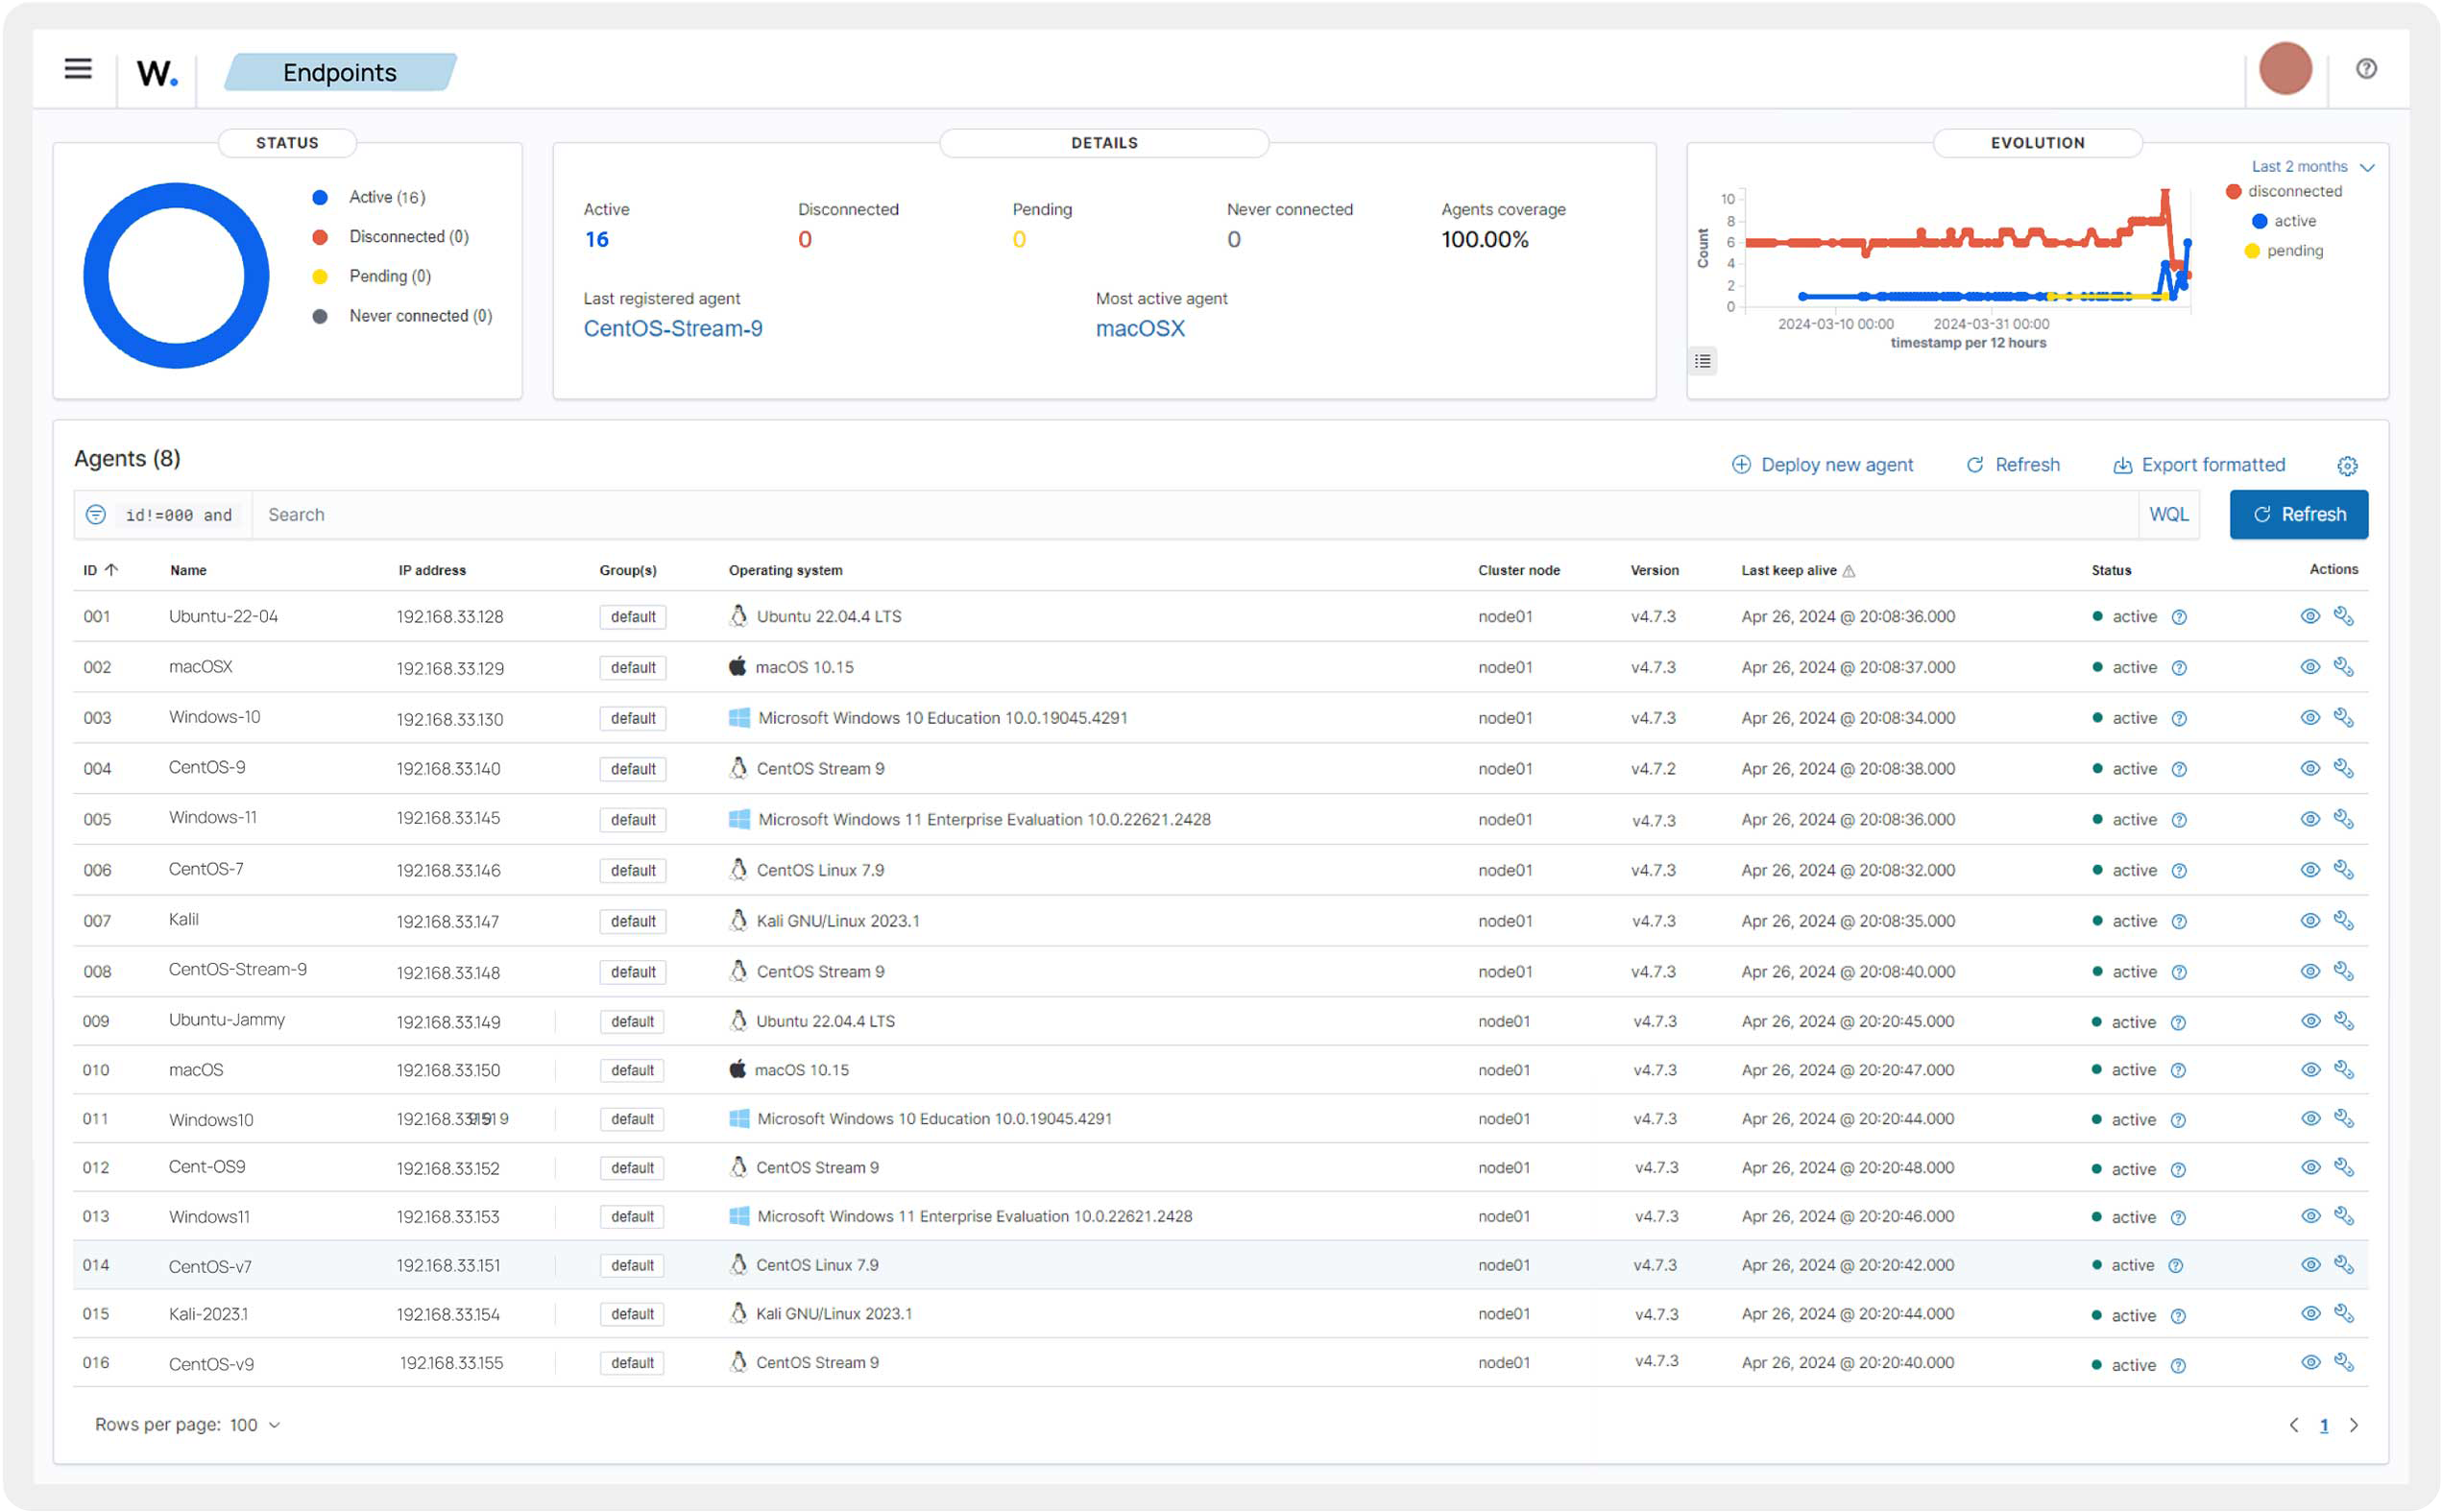
\includegraphics[width=0.9\linewidth]{images/wazuh}
	\caption{Vista referencial de Wazuh}\label{fig:wazuh}
\end{figure}

